% paper/oe_supplement.tex -- supplement to oe_main.tex (rewrite 2026-09-26).
% Uses numbers.tex macros throughout. Evidence classes as in the main text:
% [L] literature, [P] HoloForge parameter, [D] derived here, [S] simulated.
% Template note: plain article class; swap to Optica's supplemental-document
% template before submission.

\documentclass[10pt]{article}
\usepackage[margin=1in]{geometry}
\usepackage{amsmath,amssymb,graphicx,booktabs,hyperref,tabularx}
% AUTO-GENERATED by scripts/make_numbers_tex.py -- DO NOT HAND-EDIT.
% Regenerate: python scripts/make_numbers_tex.py
\usepackage{xcolor}  % for the [PENDING] flag color, harmless if already loaded

\newcommand{\MeasuredContrastTwoX}{2.00}
\newcommand{\KcPredTwoX}{4.22}
\newcommand{\KstarTwoXInterp}{4.18}
\newcommand{\KstarTwoXCI}{\textcolor{red}{[PENDING]}}
\newcommand{\MeanGainTwoX}{0.40}
\newcommand{\MinGainTwoX}{-0.03}
\newcommand{\MeasuredContrastFourX}{3.80}
\newcommand{\KcPredFourX}{6.96}
\newcommand{\KstarFourXInterp}{\textcolor{red}{[PENDING]}}
\newcommand{\KstarFourXCI}{8.98}
\newcommand{\MeanGainFourX}{0.70}
\newcommand{\MinGainFourX}{0.04}
\newcommand{\MeasuredContrastEightX}{5.32}
\newcommand{\KcPredEightX}{9.33}
\newcommand{\KstarEightXInterp}{\textcolor{red}{[PENDING]}}
\newcommand{\KstarEightXCI}{8.98}
\newcommand{\MeanGainEightX}{0.88}
\newcommand{\MinGainEightX}{0.05}
\newcommand{\MinGainAllBudgets}{-0.03}
\newcommand{\SEightGainKLowSlantZero}{0.913}
\newcommand{\SEightLoKLowSlantZero}{0.906}
\newcommand{\SEightHiKLowSlantZero}{0.920}
\newcommand{\SEightGainKLowSlantTwoFive}{3.122}
\newcommand{\SEightLoKLowSlantTwoFive}{3.122}
\newcommand{\SEightHiKLowSlantTwoFive}{3.123}
\newcommand{\SEightGainKLowSlantFive}{2.077}
\newcommand{\SEightLoKLowSlantFive}{2.076}
\newcommand{\SEightHiKLowSlantFive}{2.078}
\newcommand{\SEightGainKLowSlantSevenFive}{0.227}
\newcommand{\SEightLoKLowSlantSevenFive}{0.223}
\newcommand{\SEightHiKLowSlantSevenFive}{0.230}
\newcommand{\SEightGainKLowSlantTen}{0.089}
\newcommand{\SEightLoKLowSlantTen}{0.089}
\newcommand{\SEightHiKLowSlantTen}{0.089}
\newcommand{\SEightGainKLowSlantFifteen}{-0.007}
\newcommand{\SEightLoKLowSlantFifteen}{-0.016}
\newcommand{\SEightHiKLowSlantFifteen}{0.002}
\newcommand{\SEightGainKLowSlantTwenty}{0.024}
\newcommand{\SEightLoKLowSlantTwenty}{0.019}
\newcommand{\SEightHiKLowSlantTwenty}{0.028}
\newcommand{\SEightGainKMidSlantZero}{0.899}
\newcommand{\SEightLoKMidSlantZero}{0.898}
\newcommand{\SEightHiKMidSlantZero}{0.901}
\newcommand{\SEightGainKMidSlantTwoFive}{1.017}
\newcommand{\SEightLoKMidSlantTwoFive}{0.980}
\newcommand{\SEightHiKMidSlantTwoFive}{1.055}
\newcommand{\SEightGainKMidSlantFive}{2.045}
\newcommand{\SEightLoKMidSlantFive}{2.044}
\newcommand{\SEightHiKMidSlantFive}{2.046}
\newcommand{\SEightGainKMidSlantSevenFive}{0.291}
\newcommand{\SEightLoKMidSlantSevenFive}{0.210}
\newcommand{\SEightHiKMidSlantSevenFive}{0.371}
\newcommand{\SEightGainKMidSlantTen}{0.185}
\newcommand{\SEightLoKMidSlantTen}{0.182}
\newcommand{\SEightHiKMidSlantTen}{0.187}
\newcommand{\SEightGainKMidSlantFifteen}{0.046}
\newcommand{\SEightLoKMidSlantFifteen}{0.045}
\newcommand{\SEightHiKMidSlantFifteen}{0.046}
\newcommand{\SEightGainKMidSlantTwenty}{0.011}
\newcommand{\SEightLoKMidSlantTwenty}{0.011}
\newcommand{\SEightHiKMidSlantTwenty}{0.011}
\newcommand{\NZZeroPooledGainThirtyTwo}{0.640}
\newcommand{\NZZeroPooledLoThirtyTwo}{0.640}
\newcommand{\NZZeroPooledHiThirtyTwo}{0.640}
\newcommand{\NZZeroPooledGainOneTwentyEight}{0.641}
\newcommand{\NZZeroPooledLoOneTwentyEight}{0.641}
\newcommand{\NZZeroPooledHiOneTwentyEight}{0.641}
\newcommand{\NZZeroPooledGainTwoFiftySix}{0.645}
\newcommand{\NZZeroPooledLoTwoFiftySix}{0.645}
\newcommand{\NZZeroPooledHiTwoFiftySix}{0.645}
\newcommand{\NZZeroGainKLowThirtyTwo}{1.019}
\newcommand{\NZZeroGainKLowOneTwentyEight}{0.915}
\newcommand{\NZZeroGainKLowTwoFiftySix}{0.894}
\newcommand{\NZZeroGainKMidThirtyTwo}{0.731}
\newcommand{\NZZeroGainKMidOneTwentyEight}{0.900}
\newcommand{\NZZeroGainKMidTwoFiftySix}{0.928}
\newcommand{\SOneBaselineGain}{1.81}
\newcommand{\SOneNoSaturationGain}{2.22}
\newcommand{\SOneNoSaturationRatio}{1.2}
\newcommand{\SOneNoDiffusionRatio}{1.14}
\newcommand{\SOneNoNonlocalityRatio}{0.98}
\newcommand{\SOneNoDyeDepletionRatio}{0.98}
\newcommand{\STwoBaselineGain}{0.11}
\newcommand{\STwoGainMin}{0.08}
\newcommand{\STwoGainMax}{0.15}
\newcommand{\SThreeNominalGain}{1.81}
\newcommand{\SThreeWorstWithinFifty}{1.17}
\newcommand{\SThreeWorstWithinFiftyParam}{dn\_max}
\newcommand{\SThreeBestWithinFifty}{1.92}
\newcommand{\SThreeDnMaxFlipPct}{473}
\newcommand{\SThreeDnMaxWorstGain}{-3.73}
\newcommand{\SThreeDnMaxAtHundred}{0.99}
\newcommand{\SThreeDnMaxMostNegativePct}{-83}
\newcommand{\SThreeDnMaxAtMostNegative}{0.38}
\newcommand{\SThreeDnMaxMostPositivePct}{473}
\newcommand{\SThreeDnMaxAtMostPositive}{-3.73}
\newcommand{\SThreeAnyFlipWithinFifty}{no}
\newcommand{\SATMeanGainTwoX}{0.07}
\newcommand{\SATFracOfMILTwoX}{18}
\newcommand{\SATMeanGainFourX}{0.20}
\newcommand{\SATFracOfMILFourX}{28}
\newcommand{\SATMeanGainEightX}{0.36}
\newcommand{\SATFracOfMILEightX}{42}
\newcommand{\SATFitNRMSE}{0.103}
\newcommand{\SATFitAEff}{7.05}
\newcommand{\SATSubCliffGain}{0.98}
\newcommand{\SATSubCliffMILGain}{1.37}
\newcommand{\SATSubCliffFracOfMIL}{71}
\newcommand{\SATSubCliffFracMin}{79}
\newcommand{\SATSubCliffFracMax}{79}
\newcommand{\SATSubCliffK}{1.31}
\newcommand{\SATNearCliffK}{3.93}
\newcommand{\SATNearCliffFrac}{56}
\newcommand{\SATPostCliffK}{5.24}
\newcommand{\SATPostCliffFracMin}{-28}
\newcommand{\SATPostCliffFracMax}{-28}
\newcommand{\SeedCountMin}{3}
\newcommand{\SeedCountMax}{3}
\newcommand{\SeedCountDesc}{3}
\newcommand{\SeedCountModal}{3}
\newcommand{\SeedCountNExtraConfigs}{0}
\newcommand{\SeedCount}{3}
\newcommand{\NResultFiles}{2375}

% --- supplement macros (already-real data, not Phase-3-gated) ---
\newcommand{\AblationCheckpointCosSim}{1.000}
\newcommand{\AblationSurrogateCosSim}{0.844}
\newcommand{\RCWAMaxDevThreeCase}{0.038}
\newcommand{\RCWAVGridMaxDev}{0.980}
\newcommand{\RCWAVGridNCases}{90}
\newcommand{\RCWAUnslantedMaxDev}{0.29}
\newcommand{\RCWANormalMedianDev}{0.001}
\newcommand{\MeshPSNRSpread}{0.036}
\newcommand{\WavelengthDesignPSNR}{6.63}

% --- validation (Phase 6 / Section 6) macros ---
\newcommand{\NLiteratureSources}{3}
\newcommand{\NRMSEBruderGrowthDnKExp}{0.28}
\newcommand{\NRMSEBruderGrowthDnKSim}{0.17}
\newcommand{\NRMSEHsiehGrowthDnK}{0.10}
\newcommand{\NRMSEWorstFit}{0.28}
\newcommand{\NRMSEBestFit}{0.10}
\newcommand{\NGoodFits}{3}
\newcommand{\NRMSEWorstInRegime}{0.28}
\newcommand{\NRMSEBestInRegime}{0.17}
\newcommand{\NInRegimeSources}{2}
\newcommand{\BayfolDnMaxRatio}{5.7}

% --- baseline completeness (Sec. 5.2 / F4b) macros ---
\newcommand{\GSGainMin}{-1.27}
\newcommand{\GSGainMax}{0.00}
\newcommand{\LPCGainMin}{-1.82}
\newcommand{\LPCGainMax}{0.07}
\newcommand{\MILGainMinAtTwoX}{-0.03}

% --- shrinkage-induced shift bound (Discussion) macros ---
\newcommand{\ShrinkagePct}{0.5}
\newcommand{\ShrinkageSlantDeg}{20}
\newcommand{\ShrinkageThicknessUm}{30}
\newcommand{\ShrinkageShiftNm}{54.6}
\newcommand{\ShrinkageFracLowK}{1.7}
\newcommand{\ShrinkageFracHighK}{13.7}

% --- cost-benefit (Sec. 5.1) macros ---
\newcommand{\ComputeMatchRatio}{21.7}

% --- R1 reconstruction figure macros ---
\newcommand{\ROneSeedValue}{0}

% --- WP3 baseline (RSGD/GPC, Sec. 5.2) macros ---
\newcommand{\RSGDGainMin}{-0.00}
\newcommand{\RSGDGainMax}{0.00}
\newcommand{\GPCGainMin}{-1.98}
\newcommand{\GPCGainMax}{0.07}
\newcommand{\GPCLPCMaxAbsDiffTwoX}{0.18}

% --- WP4 (target ensemble / noise robustness, Sec. 5.x) macros ---
\newcommand{\SFourGainBarsTwoX}{0.90}
\newcommand{\SFourBootCILoBarsTwoX}{0.90}
\newcommand{\SFourBootCIHiBarsTwoX}{0.90}
\newcommand{\SFourGainBarsEightX}{1.95}
\newcommand{\SFourBootCILoBarsEightX}{1.95}
\newcommand{\SFourBootCIHiBarsEightX}{1.95}
\newcommand{\SFourGainSpotsTwoX}{3.22}
\newcommand{\SFourBootCILoSpotsTwoX}{3.19}
\newcommand{\SFourBootCIHiSpotsTwoX}{3.23}
\newcommand{\SFourGainSpotsEightX}{4.07}
\newcommand{\SFourBootCILoSpotsEightX}{3.99}
\newcommand{\SFourBootCIHiSpotsEightX}{4.12}
\newcommand{\SFourGainRandomBinaryTwoX}{0.17}
\newcommand{\SFourBootCILoRandomBinaryTwoX}{0.17}
\newcommand{\SFourBootCIHiRandomBinaryTwoX}{0.17}
\newcommand{\SFourGainRandomBinaryEightX}{0.24}
\newcommand{\SFourBootCILoRandomBinaryEightX}{0.24}
\newcommand{\SFourBootCIHiRandomBinaryEightX}{0.24}
\newcommand{\SFiveNoiseStdPct}{5}
\newcommand{\SFiveNoiselessGain}{0.90}
\newcommand{\SFiveNoisyGain}{0.88}

% --- WP5 (joint miscalibration Monte Carlo, Sec. 5.x) macros ---
\newcommand{\SSixNDraws}{30}
\newcommand{\SSixMeanGain}{1.76}
\newcommand{\SSixBootCILo}{1.73}
\newcommand{\SSixBootCIHi}{1.79}
\newcommand{\SSixNNegative}{0}
\newcommand{\SSixWorstDrawGain}{1.61}
\newcommand{\SSixBestDrawGain}{1.94}
\newcommand{\SSixPctRange}{25}

% --- WP6 (depth-resolved absorption, Sec. 5.x) macros ---
\newcommand{\SSevenGainODZero}{1.81}
\newcommand{\SSevenGainODOneTenth}{1.51}
\newcommand{\SSevenGainODThreeTenths}{1.45}

% --- PATH_TO_7 rewrite macros (complete M1 cells only) ---
\newcommand{\MOneNK}{10}
\newcommand{\MOneNCells}{30}
\newcommand{\MOneKMin}{1.96}
\newcommand{\MOneKMax}{15.71}
\newcommand{\MOneKList}{1.96, 2.62, 3.49, 3.93, 4.19, 4.83, 5.71, 6.98, 8.98, 15.71}
\newcommand{\MOneNPositive}{29}
\newcommand{\MOneNCIAboveZero}{27}
\newcommand{\MOneNCIIncludesZero}{2}
\newcommand{\MOneNNegative}{1}
\newcommand{\MOneNegK}{4.19}
\newcommand{\MOneNegBudget}{2}
\newcommand{\MOneNegGain}{-0.03}
\newcommand{\MOneNegCILo}{-0.05}
\newcommand{\MOneNegCIHi}{-0.005}
\newcommand{\MaxGainTwoX}{1.42}
\newcommand{\MaxGainKTwoX}{2.62}
\newcommand{\GainHighKTwoX}{0.01}
\newcommand{\GainHighKLoTwoX}{0.002}
\newcommand{\GainHighKHiTwoX}{0.008}
\newcommand{\MaxGainFourX}{2.13}
\newcommand{\MaxGainKFourX}{1.96}
\newcommand{\GainHighKFourX}{0.04}
\newcommand{\GainHighKLoFourX}{0.009}
\newcommand{\GainHighKHiFourX}{0.062}
\newcommand{\MaxGainEightX}{2.52}
\newcommand{\MaxGainKEightX}{2.62}
\newcommand{\GainHighKEightX}{0.05}
\newcommand{\GainHighKLoEightX}{0.019}
\newcommand{\GainHighKHiEightX}{0.091}
\newcommand{\MOneNExcluded}{0}
\newcommand{\SOneGBaselineSub}{4.41}
\newcommand{\SOneGBaselineNear}{0.90}
\newcommand{\SOneGBaselinePost}{0.11}
\newcommand{\SOneGNoSatSub}{5.39}
\newcommand{\SOneGNoSatNear}{0.61}
\newcommand{\SOneGNoSatPost}{0.66}
\newcommand{\SOneGNoDiffSub}{4.93}
\newcommand{\SOneGNoDiffNear}{1.14}
\newcommand{\SOneGNoDiffPost}{0.10}
\newcommand{\SOneGNoNonlocSub}{4.47}
\newcommand{\SOneGNoNonlocNear}{0.82}
\newcommand{\SOneGNoNonlocPost}{0.05}
\newcommand{\SOneGNoDyeSub}{4.36}
\newcommand{\SOneGNoDyeNear}{0.84}
\newcommand{\SOneGNoDyePost}{0.11}
\newcommand{\SOneKSub}{1.31}
\newcommand{\SOneKNear}{3.93}
\newcommand{\SOneKPost}{5.24}
\newcommand{\SXGBaselineSub}{4.41}
\newcommand{\SXNBaselineSub}{3}
\newcommand{\SXGBaselineNear}{0.90}
\newcommand{\SXNBaselineNear}{3}
\newcommand{\SXGBaselinePost}{0.11}
\newcommand{\SXNBaselinePost}{3}
\newcommand{\SXGNoMonomerSub}{-0.12}
\newcommand{\SXNNoMonomerSub}{3}
\newcommand{\SXGNoMonomerNear}{-0.09}
\newcommand{\SXNNoMonomerNear}{3}
\newcommand{\SXGNoMonomerPost}{-0.08}
\newcommand{\SXNNoMonomerPost}{3}
\newcommand{\SXGNoDyeSub}{4.35}
\newcommand{\SXNNoDyeSub}{3}
\newcommand{\SXGNoDyeNear}{0.84}
\newcommand{\SXNNoDyeNear}{3}
\newcommand{\SXGNoDyePost}{0.11}
\newcommand{\SXNNoDyePost}{3}
\newcommand{\SXGNoSatSub}{5.38}
\newcommand{\SXNNoSatSub}{3}
\newcommand{\SXGNoSatNear}{0.62}
\newcommand{\SXNNoSatNear}{3}
\newcommand{\SXGNoSatPost}{0.66}
\newcommand{\SXNNoSatPost}{3}
\newcommand{\SXGOnlyTanhSub}{-0.10}
\newcommand{\SXNOnlyTanhSub}{3}
\newcommand{\SXGOnlyTanhNear}{-0.02}
\newcommand{\SXNOnlyTanhNear}{3}
\newcommand{\SXGOnlyTanhPost}{-0.03}
\newcommand{\SXNOnlyTanhPost}{3}
\newcommand{\SXGOnlyDyeSub}{14.37}
\newcommand{\SXNOnlyDyeSub}{3}
\newcommand{\SXGOnlyDyeNear}{6.38}
\newcommand{\SXNOnlyDyeNear}{3}
\newcommand{\SXGOnlyDyePost}{7.40}
\newcommand{\SXNOnlyDyePost}{3}
\newcommand{\SXGOnlyMonomerSub}{5.75}
\newcommand{\SXNOnlyMonomerSub}{3}
\newcommand{\SXGOnlyMonomerNear}{1.73}
\newcommand{\SXNOnlyMonomerNear}{3}
\newcommand{\SXGOnlyMonomerPost}{1.26}
\newcommand{\SXNOnlyMonomerPost}{3}
\newcommand{\SXGLinearSub}{14.94}
\newcommand{\SXNLinearSub}{3}
\newcommand{\SXGLinearNear}{7.66}
\newcommand{\SXNLinearNear}{3}
\newcommand{\SXGLinearPost}{9.04}
\newcommand{\SXNLinearPost}{3}
\newcommand{\SXGLinearMatchedSub}{-0.00}
\newcommand{\SXNLinearMatchedSub}{3}
\newcommand{\SXGLinearMatchedNear}{0.00}
\newcommand{\SXNLinearMatchedNear}{3}
\newcommand{\SXGLinearMatchedPost}{0.10}
\newcommand{\SXNLinearMatchedPost}{3}
\newcommand{\SXGNoMonomerMatchedSub}{3.64}
\newcommand{\SXNNoMonomerMatchedSub}{3}
\newcommand{\SXGNoMonomerMatchedNear}{0.72}
\newcommand{\SXNNoMonomerMatchedNear}{3}
\newcommand{\SXGNoMonomerMatchedPost}{0.08}
\newcommand{\SXNNoMonomerMatchedPost}{3}
\newcommand{\SXGOnlyDyeMatchedSub}{1.98}
\newcommand{\SXNOnlyDyeMatchedSub}{3}
\newcommand{\SXGOnlyDyeMatchedNear}{0.42}
\newcommand{\SXNOnlyDyeMatchedNear}{3}
\newcommand{\SXGOnlyDyeMatchedPost}{-0.02}
\newcommand{\SXNOnlyDyeMatchedPost}{3}
\newcommand{\SXGOnlyTanhMatchedSub}{2.80}
\newcommand{\SXNOnlyTanhMatchedSub}{3}
\newcommand{\SXGOnlyTanhMatchedNear}{0.53}
\newcommand{\SXNOnlyTanhMatchedNear}{3}
\newcommand{\SXGOnlyTanhMatchedPost}{0.12}
\newcommand{\SXNOnlyTanhMatchedPost}{3}
\newcommand{\SXDeviceMaxDiff}{0.001}
\newcommand{\SATFracLowKMin}{36}
\newcommand{\SATFracLowKMax}{44}
\newcommand{\SATFracSecondKMin}{53}
\newcommand{\SATFracSecondKMax}{66}
\newcommand{\SATNBelowBSGD}{12}
\newcommand{\SATNCells}{29}
\newcommand{\SThreeDnMaxAtMinusFifty}{1.17}
\newcommand{\SThreeDnMaxAtPlusFifty}{1.66}
\newcommand{\MTwoRGainSub}{3.19}
\newcommand{\MTwoRLoSub}{2.94}
\newcommand{\MTwoRHiSub}{3.43}
\newcommand{\MTwoRGainNear}{0.81}
\newcommand{\MTwoRLoNear}{0.81}
\newcommand{\MTwoRHiNear}{0.81}
\newcommand{\MTwoRGainPost}{0.12}
\newcommand{\MTwoRLoPost}{0.12}
\newcommand{\MTwoRHiPost}{0.13}
\newcommand{\MTwoRSATFracSub}{79}
\newcommand{\MTwoRSATFracNear}{56}
\newcommand{\MTwoRSATFracPost}{-28}
\newcommand{\HoldoutASimIn}{0.17}
\newcommand{\HoldoutASimOut}{0.48}
\newcommand{\HoldoutASimKbleach}{\textcolor{red}{[PENDING]}}
\newcommand{\HoldoutASimDnMax}{0.0504}
\newcommand{\HoldoutASimAtBound}{none}
\newcommand{\HoldoutAExpIn}{0.28}
\newcommand{\HoldoutAExpOut}{1.09}
\newcommand{\HoldoutAExpKbleach}{\textcolor{red}{[PENDING]}}
\newcommand{\HoldoutAExpDnMax}{0.289}
\newcommand{\HoldoutAExpAtBound}{none}
\newcommand{\HoldoutBSimIn}{0.02}
\newcommand{\HoldoutBSimOut}{0.40}
\newcommand{\HoldoutBSimKbleach}{0.0667}
\newcommand{\HoldoutBSimDnMax}{0.0418}
\newcommand{\HoldoutBSimAtBound}{none}
\newcommand{\HoldoutBExpIn}{0.17}
\newcommand{\HoldoutBExpOut}{0.31}
\newcommand{\HoldoutBExpKbleach}{0.0215}
\newcommand{\HoldoutBExpDnMax}{0.0321}
\newcommand{\HoldoutBExpAtBound}{none}

% --- diffraction-efficiency confirmation (Sec. 5.1) macros ---
\newcommand{\DEMeanGainTwoX}{1.80}
\newcommand{\DEMeanGainFourX}{3.00}
\newcommand{\DEMeanGainEightX}{3.94}
\newcommand{\DEMinGainAllBudgets}{-0.251}
\newcommand{\DENNegative}{15}
\newcommand{\DENPairs}{90}

% --- wasted-media measurement (Sec. 5.4) macros ---
\newcommand{\WastedMediaThreshDB}{2}
\newcommand{\WastedMediaBSGDFrac}{37}
\newcommand{\WastedMediaMILFrac}{0}
\newcommand{\WastedMediaBSGDFracOneDB}{60}
\newcommand{\WastedMediaMILFracOneDB}{57}
\newcommand{\WastedMediaBSGDFracThreeDB}{17}
\newcommand{\WastedMediaMILFracThreeDB}{0}
\newcommand{\WastedMediaNConfigs}{30}
\newcommand{\WastedMediaGSFrac}{53}
\newcommand{\WastedMediaGSFracOneDB}{60}
\newcommand{\WastedMediaGSFracThreeDB}{33}
\newcommand{\WastedMediaLPCFrac}{47}
\newcommand{\WastedMediaLPCFracOneDB}{60}
\newcommand{\WastedMediaLPCFracThreeDB}{33}
\newcommand{\WastedMediaSATFrac}{33}
\newcommand{\WastedMediaSATFracOneDB}{60}
\newcommand{\WastedMediaSATFracThreeDB}{0}
\newcommand{\WastedMediaRSGDFrac}{37}
\newcommand{\WastedMediaRSGDFracOneDB}{60}
\newcommand{\WastedMediaRSGDFracThreeDB}{17}
\newcommand{\WastedMediaGPCFrac}{47}
\newcommand{\WastedMediaGPCFracOneDB}{60}
\newcommand{\WastedMediaGPCFracThreeDB}{30}


\title{Supplement: Media-in-the-Loop Holography}
\date{}

\begin{document}
\maketitle

% ----------------------------------------------------------------------
\section*{S1: Heuristic small-signal transfer function and $K_c$ [D]}
\label{sec:supp-s1}
\textbf{Derivation (heuristic).} Take $I(x)=I_{\text{mean}}(1+m\cos Kx)$,
$m\ll1$, neglect dye depletion ($d\approx1$) and hold $D_{\text{eff}}=D_0$
(linearization about the start of recording). The uniform fields obey
$\dot u_0=-F_0u_0$ with $F_0=\kappa I_{\text{mean}}^\gamma$. Eliminating the
first-order Fourier component quasi-statically gives
\[
H(K)=\frac{\exp(-K^2\sigma^2/2)}{1+D_0K^2/F_0},
\]
implemented as \texttt{NPDDRecorder.small\_signal\_mtf}. A compensation limit
follows if the required pre-boost $1/H(K)$ exceeds the contrast budget.

\textbf{Status.} We checked this closed form against the simulator and it
does not match it; an independent numerical linearization of the same
equations does. $H(K)$ is therefore a heuristic that motivated the
hypothesis, not a validated transfer function, and no main-text result
depends on its being exact. LPC (main text, Section~4) uses it and does not
improve on media-blind SGD beyond \LPCGainMax\,dB [S].

\textbf{Definition used for $K_c$.} The pipeline compares $1/H(K)$ with the
contrast the optimizer actually realized at each grid $K$ (not the nominal
budget) and reports the smallest $K$ at which $1/H$ exceeds it, linearly
interpolated. Mean realized contrast is \MeasuredContrastTwoX,
\MeasuredContrastFourX{} and \MeasuredContrastEightX{} at nominal budgets
2, 4 and 8, giving $K_c=\KcPredTwoX$, \KcPredFourX{} and
\KcPredEightX\,rad/\textmu m. At budget 8 the optimizer does not realize
the nominal contrast at several $K$, which is why $K_c$ grows less than the
nominal budget would suggest.

\begin{figure}[htbp]
\centering
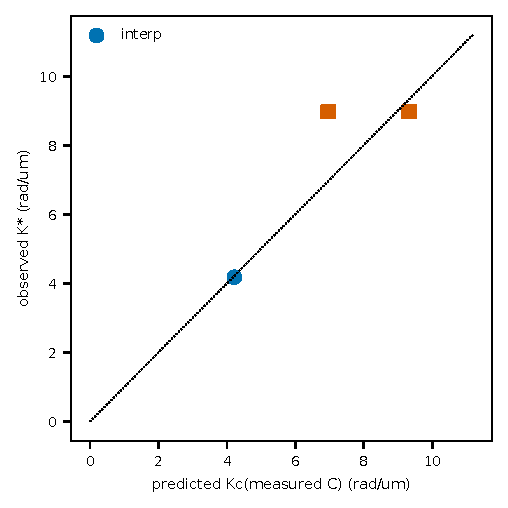
\includegraphics[width=0.65\linewidth]{../code/figures/paper/F5_Kstar_vs_Kc_scatter.pdf}
\caption{Observed $K^*$ estimators vs.\ heuristic $K_c$. The zero-crossing
estimator returns a point only at budget 2 ($K^*=\KstarTwoXInterp$); the
CI-based estimator marks where the interval first includes zero and stays
small, i.e.\ the onset of the high-$K$ plateau.}
\end{figure}

\textbf{Exposure and index profiles behind main-text Fig.~R1.}
\begin{figure}[htbp]
\centering
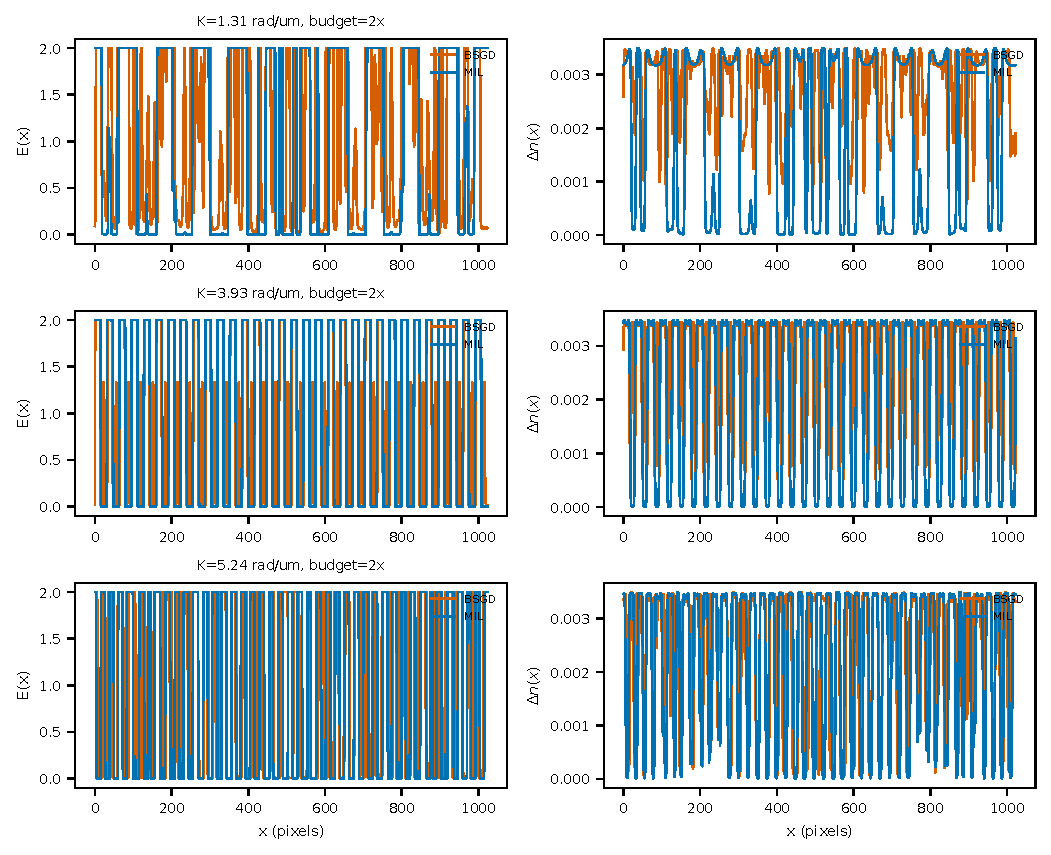
\includegraphics[width=0.85\linewidth]{../code/figures/paper/R3_exposure_profiles.pdf}
\caption{Exposure $E(x)$ (left) and recorded $\Delta n(x)$ (right), BSGD vs.\
MIL, same $K$, budget and seed as main-text Fig.~R1 [S].}
\end{figure}
In these single-seed examples BSGD's linear assumption drives $E(x)$ towards
near-binary swings, which at the higher $K$ push $\Delta n(x)$ towards
$\Delta n_{\max}$ over most of the period; MIL's exposure is less extreme.
This is an illustration of one seed, not a statistical claim.

% ----------------------------------------------------------------------
\section*{S2: Mechanism ablations [S]}
\label{sec:supp-s2}
\textbf{One at a time.} Conditions: $\sigma\to0$ (no non-locality),
$D_0\to0$ (no diffusion), $k_{\text{bleach}}\to0$ (no dye depletion), and the
$\tanh$ index map replaced by its linear limit $\Delta n=1.5\,\Delta n_{\max}N$
(no index saturation). An earlier version approximated the last by scaling
$\Delta n_{\max}$ by $100\times$, which leaves $N$ and the $\tanh$ saturation
unchanged and therefore did not remove saturation; it was replaced.
Values are in main-text Table~2; Fig.~S2a shows them with intervals.

\begin{figure}[htbp]
\centering
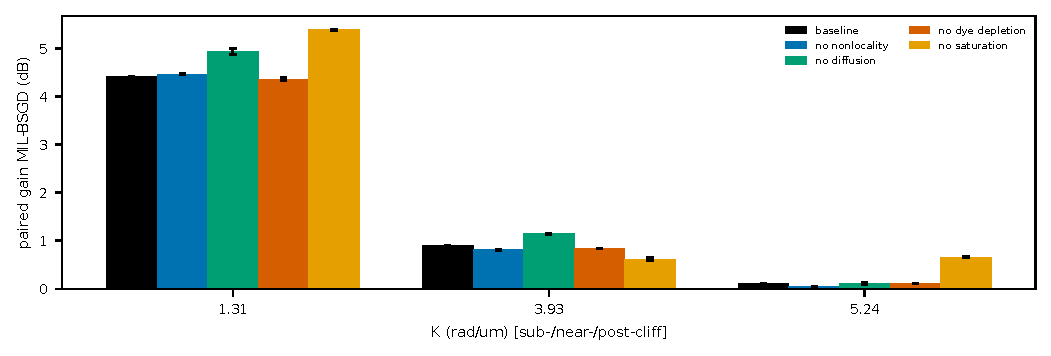
\includegraphics[width=\linewidth]{../code/figures/paper/F7_physics_ablation.pdf}
\caption{S2a: paired gain by single-mechanism ablation at three $K$, budget
2, 95\% $t$-intervals over three seeds.}
\end{figure}

\textbf{Factorial over the saturating mechanisms.} M = monomer depletion
(removed by holding $u\equiv1$: polymer production continues at the local
rate, the reservoir never empties), D = dye bleaching ($k_{\text{bleach}}=0$),
T = $\tanh$ index map (linearized). ``Matched'' rows rescale $\kappa$ so that
the cured polymer at unit uniform dose is $N=1$, as in the full model:
$\kappa=0.2/(1-e^{-2})$ when bleaching is on and $\kappa=0.1$ when it is off
[D]. ``Linear, slope-matched'' sets $\kappa=1/15$ with all three removed, so
that $\Delta n=\Delta n_{\max}(G_\sigma*E)$, the media-blind model up to blur
and shrinkage [D]. Jobs ran on CPU (float32); the full-model row reproduces
the GPU values of main-text Table~2 to within \SXDeviceMaxDiff\,dB.

\begin{center}
\begin{tabular}{llccc}
\toprule
Active & Condition & $K=\SOneKSub$ & $K=\SOneKNear$ & $K=\SOneKPost$ \\
\midrule
M D T & full model & \SXGBaselineSub & \SXGBaselineNear & \SXGBaselinePost \\
\phantom{M} D T & no monomer depletion & \SXGNoMonomerSub & \SXGNoMonomerNear & \SXGNoMonomerPost \\
 & \quad matched & \SXGNoMonomerMatchedSub & \SXGNoMonomerMatchedNear & \SXGNoMonomerMatchedPost \\
M \phantom{D} T & no dye depletion & \SXGNoDyeSub & \SXGNoDyeNear & \SXGNoDyePost \\
M D \phantom{T} & no index saturation & \SXGNoSatSub & \SXGNoSatNear & \SXGNoSatPost \\
\phantom{M D} T & only $\tanh$ & \SXGOnlyTanhSub & \SXGOnlyTanhNear & \SXGOnlyTanhPost \\
 & \quad matched & \SXGOnlyTanhMatchedSub & \SXGOnlyTanhMatchedNear & \SXGOnlyTanhMatchedPost \\
\phantom{M} D \phantom{T} & only dye & \SXGOnlyDyeSub & \SXGOnlyDyeNear & \SXGOnlyDyePost \\
 & \quad matched & \SXGOnlyDyeMatchedSub & \SXGOnlyDyeMatchedNear & \SXGOnlyDyeMatchedPost \\
M \phantom{D T} & only monomer depletion & \SXGOnlyMonomerSub & \SXGOnlyMonomerNear & \SXGOnlyMonomerPost \\
-- & linear & \SXGLinearSub & \SXGLinearNear & \SXGLinearPost \\
-- & linear, slope-matched & \SXGLinearMatchedSub & \SXGLinearMatchedNear & \SXGLinearMatchedPost \\
\bottomrule
\end{tabular}
\end{center}

\begin{figure}[htbp]
\centering
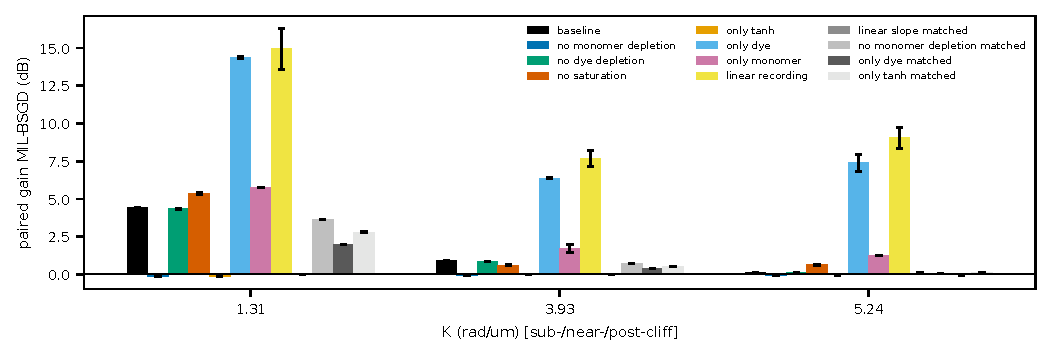
\includegraphics[width=\linewidth]{../code/figures/paper/F12_mechanism_factorial.pdf}
\caption{S2b: paired gain for every factorial condition at three $K$,
budget 2, 95\% $t$-intervals over seeds.}
\end{figure}

% ----------------------------------------------------------------------
\section*{S3: Readout slice count and grating slant [S]}
\label{sec:supp-s3}
\textbf{Slice count} (one seed, budget 2, unslanted):
\begin{center}
\begin{tabular}{lccc}
\toprule
$K$ (rad/\textmu m) & $n_z=32$ & $n_z=128$ & $n_z=256$ \\
\midrule
1.96 & \NZZeroGainKLowThirtyTwo & \NZZeroGainKLowOneTwentyEight & \NZZeroGainKLowTwoFiftySix \\
3.93 & \NZZeroGainKMidThirtyTwo & \NZZeroGainKMidOneTwentyEight & \NZZeroGainKMidTwoFiftySix \\
pooled over three $K$ & \NZZeroPooledGainThirtyTwo & \NZZeroPooledGainOneTwentyEight & \NZZeroPooledGainTwoFiftySix \\
\bottomrule
\end{tabular}
\end{center}
All experiments use $n_z=128$. An earlier version of this study used
$n_z=32$, which is not converged at $K=3.93$.

\textbf{Slant} (budget 2, three seeds, mean and 95\% $t$-interval):
\begin{center}
\small
\begin{tabular}{lccccccc}
\toprule
$\phi$ & $0^\circ$ & $2.5^\circ$ & $5^\circ$ & $7.5^\circ$ & $10^\circ$ & $15^\circ$ & $20^\circ$ \\
\midrule
$K=1.96$ & \SEightGainKLowSlantZero & \SEightGainKLowSlantTwoFive & \SEightGainKLowSlantFive & \SEightGainKLowSlantSevenFive & \SEightGainKLowSlantTen & \SEightGainKLowSlantFifteen & \SEightGainKLowSlantTwenty \\
 & {\scriptsize[\SEightLoKLowSlantZero, \SEightHiKLowSlantZero]} & {\scriptsize[\SEightLoKLowSlantTwoFive, \SEightHiKLowSlantTwoFive]} & {\scriptsize[\SEightLoKLowSlantFive, \SEightHiKLowSlantFive]} & {\scriptsize[\SEightLoKLowSlantSevenFive, \SEightHiKLowSlantSevenFive]} & {\scriptsize[\SEightLoKLowSlantTen, \SEightHiKLowSlantTen]} & {\scriptsize[\SEightLoKLowSlantFifteen, \SEightHiKLowSlantFifteen]} & {\scriptsize[\SEightLoKLowSlantTwenty, \SEightHiKLowSlantTwenty]} \\
$K=3.93$ & \SEightGainKMidSlantZero & \SEightGainKMidSlantTwoFive & \SEightGainKMidSlantFive & \SEightGainKMidSlantSevenFive & \SEightGainKMidSlantTen & \SEightGainKMidSlantFifteen & \SEightGainKMidSlantTwenty \\
 & {\scriptsize[\SEightLoKMidSlantZero, \SEightHiKMidSlantZero]} & {\scriptsize[\SEightLoKMidSlantTwoFive, \SEightHiKMidSlantTwoFive]} & {\scriptsize[\SEightLoKMidSlantFive, \SEightHiKMidSlantFive]} & {\scriptsize[\SEightLoKMidSlantSevenFive, \SEightHiKMidSlantSevenFive]} & {\scriptsize[\SEightLoKMidSlantTen, \SEightHiKMidSlantTen]} & {\scriptsize[\SEightLoKMidSlantFifteen, \SEightHiKMidSlantFifteen]} & {\scriptsize[\SEightLoKMidSlantTwenty, \SEightHiKMidSlantTwenty]} \\
\bottomrule
\end{tabular}
\end{center}
Slanted values rely on the scalar readout outside the geometry in which it
was checked against RCWA (S5) and are model-dependent.

% ----------------------------------------------------------------------
\section*{S4: One-parameter miscalibration [S]}
\label{sec:supp-s4}
The exposure is designed on the nominal twin and scored unchanged on a twin
with one of $D_0$, $\sigma$, $\kappa$, $\Delta n_{\max}$ perturbed (three $K$,
budget 2, $K$-averaged per seed, then 95\% interval over seeds).
\begin{figure}[htbp]
\centering
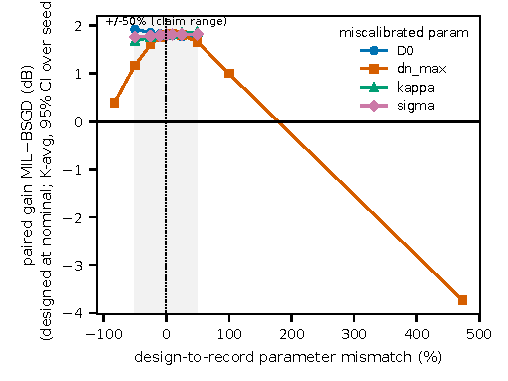
\includegraphics[width=0.8\linewidth]{../code/figures/paper/F10_twin_mismatch.pdf}
\caption{Paired gain vs.\ design-to-recording parameter error. Shading: the
$\pm50\%$ range. $\Delta n_{\max}$ is swept to $\SThreeDnMaxMostNegativePct\%$
and $+\SThreeDnMaxMostPositivePct\%$ to bracket the disagreement between our
two Bayfol fits.}
\end{figure}
Within $\pm50\%$ the gain stays between \SThreeWorstWithinFifty{} and
\SThreeBestWithinFifty\,dB, the lowest value belonging to
\SThreeWorstWithinFiftyParam. For $\Delta n_{\max}$: \SThreeDnMaxAtMostNegative\,dB
at $\SThreeDnMaxMostNegativePct\%$, \SThreeDnMaxAtHundred\,dB at $+100\%$,
\SThreeDnMaxAtMostPositive\,dB at $+\SThreeDnMaxMostPositivePct\%$. The
grid has no points between $+100\%$ and $+\SThreeDnMaxMostPositivePct\%$, so
where the sign changes is not resolved.

% ----------------------------------------------------------------------
\section*{S5: RCWA check of the closed-form readout [S]}
\label{sec:supp-s5}
Kogelnik first-order efficiency~\cite{kogelnik1969coupled} was compared with
RCWA~\cite{moharam1981rigorous} (TORCWA~\cite{kim2023torcwa}). A 3-case
check (TE, unslanted, near-Bragg) agrees to \RCWAMaxDevThreeCase{} absolute
efficiency; the \RCWAVGridNCases-case grid (TE and TM, three geometries,
several $\Delta n$ and $K$) gives at most \RCWAUnslantedMaxDev{} for
unslanted geometries and up to \RCWAVGridMaxDev{} for a $20^\circ$ slant,
concentrated at high $K$ where the slant detunes the Bragg condition.
\begin{figure}[htbp]
\centering
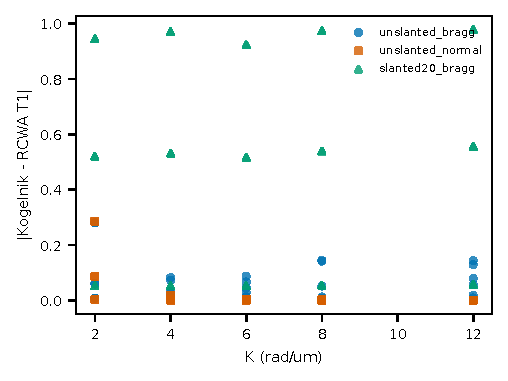
\includegraphics[width=0.8\linewidth]{../code/figures/paper/F3a_rcwa_validity_envelope.pdf}
\caption{$|\eta_{\text{Kogelnik}}-\eta_{\text{RCWA}}|$ across the grid, one
series per geometry.}
\end{figure}
This checks the closed-form reference, not the BPM in the design loop
directly; the two share the scalar approximation, which is why the headline
claims are restricted to unslanted gratings.

% ----------------------------------------------------------------------
\section*{S6: Compute-matched control [S]}
\label{sec:supp-s6}
BSGD receives $\lceil 800\times\ComputeMatchRatio\rceil$ iterations; MIL keeps
800. The ratio is one wall-clock measurement of per-iteration cost, not a
FLOP count. Budget 2, three seeds, three $K$ (reduced from the planned
three budgets for compute reasons).
\begin{center}
\begin{tabular}{lccc}
\toprule
 & $K=\SOneKSub$ & $K=\SOneKNear$ & $K=\SOneKPost$ \\
\midrule
MIL $-$ BSGD (compute-matched) & \MTwoRGainSub & \MTwoRGainNear & \MTwoRGainPost \\
95\% interval & [\MTwoRLoSub, \MTwoRHiSub] & [\MTwoRLoNear, \MTwoRHiNear] & [\MTwoRLoPost, \MTwoRHiPost] \\
SAT as \% of MIL & \MTwoRSATFracSub & \MTwoRSATFracNear & \MTwoRSATFracPost \\
\bottomrule
\end{tabular}
\end{center}

% ----------------------------------------------------------------------
\section*{S7: Calibrating the twin for a new medium}
\label{sec:supp-s7}
From the fits of main-text Section~6: (i) $\kappa$ and $\Delta n_{\max}$ are
identifiable from one $\Delta n_1$(dose) curve (NRMSE
\NRMSEBestInRegime--\NRMSEWorstInRegime{} here [S]); (ii) $D_0$ and $\sigma$
act through the spatial-frequency dependence and need a multi-$K$ family or
an independent measurement -- using $D_0$ in place of $\Delta n_{\max}$ as
the second free parameter produced our initial poor fits; (iii)
$\Delta n_{\max}$ must come from the same experimental condition as the
curve being fitted: our configuration had imported it from a separate
dye-screening experiment in the same source; (iv) the dose-to-time mapping
and $k_{\text{bleach}}$ are coupled, so either fit $k_{\text{bleach}}$ (as
in the held-out test) or recover the source's intensity.

% ----------------------------------------------------------------------
\section*{S8: Target content and readout noise [S]}
\label{sec:supp-s8}
At $K=3.93$\,rad/\textmu m, three target families (bars, sparse random spots,
random binary), budgets 2 and 8, three seeds, bootstrap 95\%
intervals~\cite{efron1993bootstrap}:
\begin{center}
\begin{tabular}{lcc}
\toprule
Target & budget 2 & budget 8 \\
\midrule
bars & \SFourGainBarsTwoX{} [\SFourBootCILoBarsTwoX, \SFourBootCIHiBarsTwoX] & \SFourGainBarsEightX{} [\SFourBootCILoBarsEightX, \SFourBootCIHiBarsEightX] \\
spots & \SFourGainSpotsTwoX{} [\SFourBootCILoSpotsTwoX, \SFourBootCIHiSpotsTwoX] & \SFourGainSpotsEightX{} [\SFourBootCILoSpotsEightX, \SFourBootCIHiSpotsEightX] \\
random binary & \SFourGainRandomBinaryTwoX{} [\SFourBootCILoRandomBinaryTwoX, \SFourBootCIHiRandomBinaryTwoX] & \SFourGainRandomBinaryEightX{} [\SFourBootCILoRandomBinaryEightX, \SFourBootCIHiRandomBinaryEightX] \\
\bottomrule
\end{tabular}
\end{center}
Gaussian detector noise at \SFiveNoiseStdPct\% of the reconstructed peak,
applied identically to every method before scoring: \SFiveNoiselessGain\,dB
noiseless, \SFiveNoisyGain\,dB noisy (budget 2). With three seeds, bootstrap
intervals are coarse; they are reported alongside, not instead of, the
$t$-intervals used elsewhere.

% ----------------------------------------------------------------------
\section*{S9: Implementation notes and legacy diagnostics}
\label{sec:supp-s9}
\textbf{Non-local kernel.} An earlier implementation applied $G_\sigma$ to
$u$ ($F\cdot(G_\sigma*u)$) rather than to the production term; this was
corrected before any reported result was generated.

\textbf{Conservation.} The explicit reaction step caps consumed monomer at
the available monomer, so $u\ge0$ and $u+N$ is conserved to rounding error at
any step size; an earlier version clamped $u$ after the update, which
created polymer from no monomer at large $\kappa\,\mathrm{d}t$.

\textbf{Legacy diagnostics (not used in any main-text claim; produced before
the 2026-09-19 geometry freeze).} Gradient pathways: checkpointed adjoint
cosine similarity \AblationCheckpointCosSim, neural surrogate
\AblationSurrogateCosSim. Mesh density: PSNR spread \MeshPSNRSpread\,dB over
$n_x=512$--$2048$ at a fixed window (single seed). Wavelength detuning: the
design-wavelength reconstruction scores \WavelengthDesignPSNR\,dB and falls
off non-monotonically over 400--450\,nm (single seed).

% ----------------------------------------------------------------------
\section*{S10: Claim provenance}
\label{sec:supp-s10}
Every number in the main text is a macro in \texttt{numbers.tex}, generated
by \texttt{scripts/make\_numbers\_tex.py} (plus
\texttt{analysis/de\_confirmation.py} and \texttt{analysis/wasted\_media.py})
from \texttt{results/summary/paper\_numbers.json}, which
\texttt{analysis/aggregate.py} computes from the per-job files
\texttt{results/\{tier\}/\{config\_hash\}/\{method\}\_seed\{n\}.json}. Each
job file records its configuration, git commit and device.

\begin{center}
\small
\begin{tabularx}{\linewidth}{p{0.26\linewidth} l X}
\toprule
Claim & Class & Source \\
\midrule
NPDD equations, BPM, angular spectrum, Kogelnik, Klein--Cook, RCWA, GS, Adam, AD & [L] & cited at first use \\
Medium parameters, $\beta$, grid, iterations, budgets, $n_z$, slant & [P] & Table~1; \texttt{experiments/manifest.py} \\
$H(K)$, $K_c$, LPC, GPC, SAT model, matched $\kappa$ values & [D] & S1, S2; \texttt{holomedia/}, \texttt{analysis/aggregate.py} \\
Paired gain on the grid, failure rates, DE & [S] & tier M1; \texttt{aggregate.py}, \texttt{wasted\_media.py}, \texttt{de\_confirmation.py} \\
Baselines, SAT fractions & [S] & tier M1 \\
Compute-matched arm & [S] & tier M2 (M2R subset) \\
Ablation, factorial & [S] & tiers S1, S1X \\
Slant, slice count & [S] & tiers S8, NZ0 \\
Miscalibration, joint, depth & [S] & tiers S3, S6, S7 (\texttt{experiments/run\_s*.py}) \\
Targets, noise & [S] & tiers S4, S5 (reuse M1 at $K=3.93$) \\
Twin fits, held-out prediction & [S] on [L] data & \texttt{experiments/fit\_literature\_curves.py}, \texttt{fit\_twin\_holdout.py}; \texttt{data/literature/} \\
RCWA envelope & [S] & \texttt{experiments/rcwa\_crosscheck.py} \\
\bottomrule
\end{tabularx}
\end{center}

% ----------------------------------------------------------------------
\section*{S11: Changes from the previous draft}
\label{sec:supp-s11}
The previous draft's results predated fixes to the readout (slant shear,
phase precision), the NPDD conservation step and the slice count, and were
regenerated. The following earlier statements are withdrawn because the
regenerated data do not support them:
\begin{itemize}
\item ``Saturation, not transport kinetics, is the binding constraint'': the
$K$-resolved ablation (main-text Table~2) shows no single mechanism whose
removal explains the gain.
\item ``Gain is never negative'': one grid cell is negative
(\MOneNegGain\,dB at $K=\MOneNegK$, budget \MOneNegBudget).
\item ``15 tested spatial frequencies'': the completed grid has \MOneNK.
\item ``Diffraction efficiency tells the same story with one negative pair'':
\DENNegative{} of \DENPairs{} pairs are negative.
\item The saturation-only surrogate as a general ``real competitor'': it
helps only at the two lowest $K$.
\item A headline gain of about 1\,dB at the previously stated $20^\circ$
slant: that value came from an effectively unslanted readout; at a
correctly sheared $20^\circ$ slant the gain is near zero (S3).
\end{itemize}

\bibliographystyle{unsrt}
\bibliography{refs}

\end{document}
